% \section{Introduction}

% \begin{figure*}[t]
% \centering
% 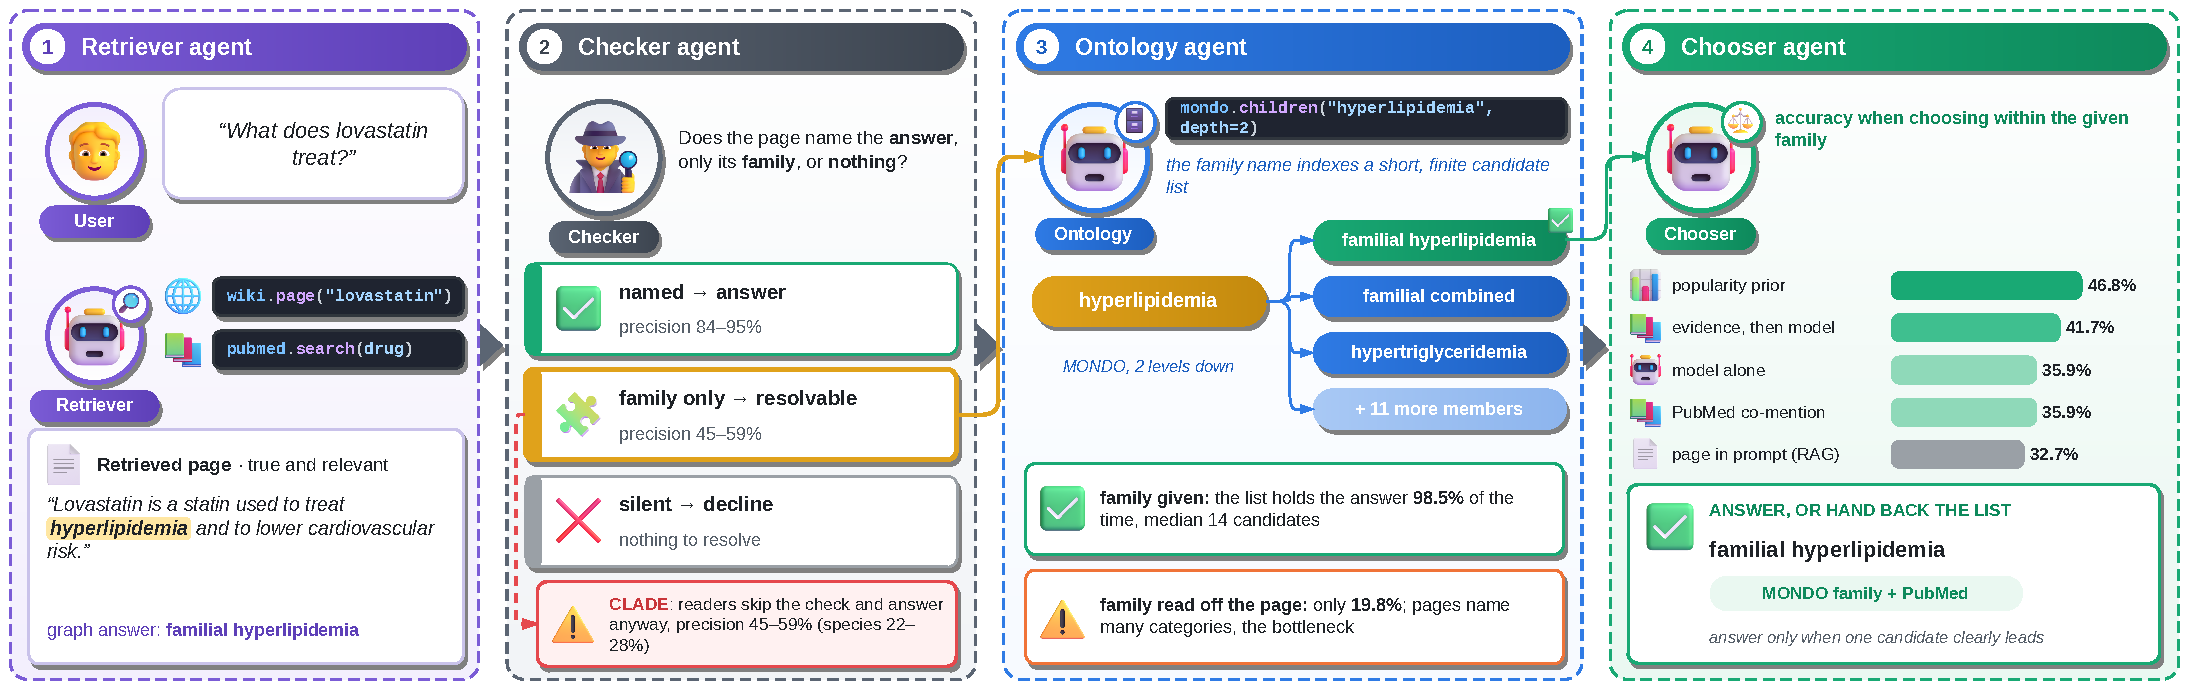
\includegraphics[width=\textwidth]{fig_concept.pdf}
% \caption{Resolvable insufficiency, drawn as a proposed agent workflow with the
% bottleneck we measure at each step. The dashed red path is \clade{}: the reader
% answers from the family-only page instead of handing it on. The retrieved page is true and relevant but
% names only the answer's family. A page-type check should route it away from
% answering; an ontology step turns the family name into a short candidate list;
% a chooser picks from it or hands the list back. Only the ontology step works
% reliably today.}
% \label{fig:concept}
% \end{figure*}

% A retrieval-augmented system answers a question by reading a page
% \citep{lewis2020rag}. Much recent work asks what the model should do when the
% page is not enough. The usual framing is binary: the context is sufficient or
% it is not \citep{joren2025sufficient}, and a well-behaved model answers in the
% first case and abstains in the second \citep{wen2025abstention}.

% Many pages fall between these cases in a structured way. Consider the question
% ``What does lovastatin treat?'' with the answer \emph{familial
% hyperlipidemia}, and a page that says ``lovastatin is used to treat
% hyperlipidemia'' (Figure~\ref{fig:concept}). The page is true and relevant. It
% rules out every disease that is not a hyperlipidemia. It does not say which
% one. A model can answer anyway, say ``not enough information,'' or look
% further. Looking further has a natural symbolic form: a disease ontology lists
% the members of the family, and each can be checked.

% We call this case \emph{resolvable insufficiency}. The page is insufficient,
% because it cannot settle the answer. It is resolvable in the sense of candidate-space reduction: the family name
% it does contain indexes a short, finite candidate set in a knowledge
% structure. Whether a system can then pick the right member is a separate
% question, which we also measure. When a model answers from such a page anyway,
% we call the behavior \clade{}: category-level answering from deficient
% evidence. This is the point where a neural reader and a symbolic resource
% have the most to offer each other, and it is common: in our data, text names
% the exact disease for only a minority of graph facts, and part of the rest is
% written at the family level.

% We ask three questions. How much of a biomedical knowledge graph does text
% name, and does a family name help a model at all? When a page names only the
% family, does a model stop declining, and are the answers it gives instead
% right? And can an ontology turn the family name back into the answer?

% Our contributions are:
% \begin{itemize}
% \item We define resolvable insufficiency and the failure it invites, \clade{},
% and measure it per fact, by
% classifying each page as naming the answer, naming only its family in the
% MONDO disease ontology, or naming nothing.
% \item We show that, pooled over three 7--8B models from different families, a
% family-only page weakens abstention relative to a silent page, using a design
% that compares each question with itself with and without the page, and that
% the answers it frees are about as often wrong as right, far less reliable than
% answers from a page that names the disease.
% \item We isolate the cause with a counterfactual edit of the same pages, show
% that confidence thresholds, a larger model and an instruction to decline do not
% remove the effect, and replicate it on species interactions with a taxonomy.
% \item We decompose ontology-based recovery into finding the family, listing
% its members, and choosing among them, and show that the first step is the
% bottleneck, while a popularity prior is a strong baseline for the last.
% \end{itemize}





\section{Introduction}

\begin{figure*}[t]
\centering
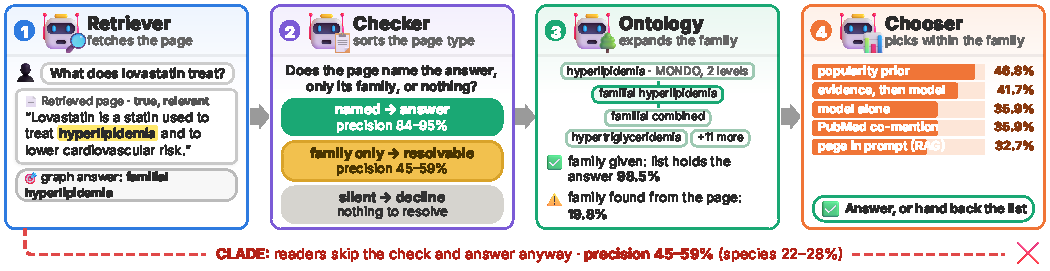
\includegraphics[width=\textwidth]{figures/fig_workflow.pdf}
\caption{\emph{Resolvable insufficiency} as an agent workflow, with the bottleneck we measure at each stage. The retrieved passage is accurate and relevant but names only the answer's family. A page-type check should send it to an ontology, which expands the family into a short candidate list for a chooser. The dashed red path is \clade{}: the model guesses from the family-only passage instead. Today only the ontology step works reliably.}
\label{fig:concept}
\end{figure*}

% Retrieval-augmented generation (RAG) systems answer questions by reading retrieved text \citep{lewis2020rag}. Recent works ask what a model should do when the retrieved text does not contain the complete answer. The usual framing is binary: the context is sufficient or it is not \citep{joren2025sufficient}, and a well-behaved model answers in the first case and abstains in the second \citep{wen2025abstention}. In practice, many retrieved passages fall between these two extremes. Consider the question, \emph{What disease does lovastatin treat?}, where the ground-truth answer is the specific condition \emph{familial hyperlipidemia}. Suppose the retriever returns a passage stating that \emph{lovastatin is used to treat hyperlipidemia} (~\ref{fig:concept}). This passage is both accurate and relevant. It rules out every disease outside the hyperlipidemia family, but it is too coarse to specify which exact subtype is meant. Faced with this passage, a system can guess a specific disease, abstain by saying there is not enough information, or look further. Looking further has a natural symbolic solution: a medical ontology lists the specific diseases within the hyperlipidemia family, and each candidate can then be checked.

% We call this phenomenon \emph{resolvable insufficiency}. The passage is insufficient on its own because it states the answer at a coarse category level rather than the fine-grained entity level required. However, it is resolvable because the coarse name maps directly to a small, finite set of candidate answers in a structured ontology. When a language model instead guesses a fine-grained answer directly from such coarse text, we call the behavior \clade{} (Category-Level Answering from Deficient Evidence). This setting represents a natural handoff point between neural readers and symbolic knowledge bases, and it occurs frequently in real text. In biomedical datasets, retrieved documents state the exact disease name for only a small fraction of knowledge-graph facts, while many of the remaining facts are described only at a broader family level. To facilitate our analysis, we group retrieved passages into three categories based on how specifically they describe the target answer:
% \begin{itemize}
% \item \emph{Named (exact-match) passages}, which explicitly mention the fine-grained target entity or an exact synonym.
% \item \emph{Family-only (coarse) passages}, which do not mention the specific answer, but mention a broader parent category (such as a disease family or biological genus) within two levels above the answer in an ontology.
% \item \emph{Silent (unmentioned) passages}, which talk about the query subject (e.g., the drug) but mention neither the specific answer nor its broader family.
% \end{itemize}

% \noindent Using the framework, we investigate three research questions:
% \begin{enumerate}
% \item How often do reference texts state fine-grained biomedical facts versus only coarse categories, and does a coarse category name help a language model answer on its own?
% \item When a retrieved passage provides only a coarse family name, does the model stop abstaining, and are the resulting answers accurate?
% \item Can a domain ontology bridge the gap by turning a coarse family mention into the exact fine-grained answer?
% \end{enumerate}

% Our main contributions are as follows:
% \begin{itemize}
% \item We define \emph{resolvable insufficiency} and the failure mode it triggers (\clade{}), and we measure how often reference texts describe knowledge-graph facts at an exact, coarse (\emph{family-only}), or unmentioned (\emph{silent}) level.
% \item Across three 7--8B language models from different model families, we show that coarse, family-only passages significantly reduce abstention compared to silent passages. By comparing each question against itself with and without the passage, we show that the extra answers triggered by family-only passages are wrong about half the time—far less reliable than answers based on named passages.
% \item We prove causality through counterfactual page edits, show that confidence filtering, larger model scale (14B), and explicit abstention prompts fail to prevent \clade{}, and replicate our findings in ecology using species interactions and a biological taxonomy.
% \item We break ontology-guided recovery into three steps—identifying the family on the page, listing its members, and selecting the final candidate—and show that identifying the right family on the page is the main bottleneck, while a simple popularity prior outperforms both the language model and literature co-mention counts at the final selection step.
% \end{itemize}


Retrieval-augmented generation (RAG) systems answer questions by reading retrieved text \citep{lewis2020rag}. Recent work asks what a model should do when that text does not contain the complete answer. The usual framing is binary: a passage is either sufficient or insufficient \citep{joren2025sufficient}, and a reliable model answers in the first case and abstains in the second \citep{wen2025abstention}. In practice, many retrieved passages fall between these two extremes. Consider the question \emph{What disease does lovastatin treat?}, where the true answer is the specific condition \emph{familial hyperlipidemia}. Suppose the retriever returns a passage stating that \emph{lovastatin is used to treat hyperlipidemia} (~\cref{fig:concept}). This passage is accurate and relevant. It rules out every disease outside the hyperlipidemia family, but it is too coarse to specify which exact subtype is meant. In this case, a system can guess a specific disease, abstain, or look further using a medical ontology that lists specific members of the hyperlipidemia family.

We call this phenomenon \emph{resolvable insufficiency}. The passage is insufficient on its own because it states the answer at a coarse category level rather than the required fine-grained entity level. Yet it is resolvable because the coarse name maps directly to a short, finite set of candidate answers in a structured ontology. When a model instead guesses a fine-grained answer directly from such coarse text, we name the behavior \clade{} (Category-Level Answering from Deficient Evidence). Although this setting occurs frequently in real text---biomedical documents state the exact disease name for only a small fraction of knowledge-graph facts while describing many others at the family level—prior work overlooks how coarse evidence affects model abstention. Rather than proposing a surface-level patch, this paper digs into the mechanics of this phenomenon to understand how coarse evidence misleads large language models (LLMs) and where a neural reader should hand off to symbolic knowledge.

To study this systematically, we group retrieved passages into three categories based on how specifically they describe the target answer: \emph{named} (exact-match) passages, which explicitly mention the fine-grained target entity or an exact synonym; \emph{family-only} (coarse) passages, which omit the specific answer but mention a broader parent category (such as a disease family or biological genus) within two levels above the answer in an ontology; and \emph{silent} (unmentioned) passages, which discuss the query subject (e.g., the drug) but mention neither the specific answer nor its broader family. Using this framework, we investigate three research questions: (1) how often reference texts state fine-grained biomedical facts versus coarse categories (and whether a coarse name helps a model on its own), (2) whether family-only passages cause models to stop abstaining and guess inaccurately, and (3) whether a domain ontology can turn a coarse family mention into the exact fine-grained answer. Our main contributions are as follows:
\begin{itemize}
\item We define \emph{resolvable insufficiency} and \clade{}, and measure how text states 1,800 PrimeKG facts and 23,694 GloBI interactions. Text omits the exact disease for 77.5--84.9\% of PrimeKG facts, and a family name alone gives the model no closed-book advantage.
\item On 856 PrimeKG questions and three 7--8B models, family-only passages cut abstention by 13.8 points relative to silent passages. About half of the extra answers are wrong, and precision falls from 84--95\% to 45--59\%.
\item Counterfactual edits show that the family name causes this drop ($-17.4$ points against deleting the sentence). Confidence filtering, a 14B model and an instruction to abstain do not stop \clade{}, and the effect replicates on 900 GloBI questions. In free text, no model gives the exact answer from a family-only passage.
\item On 410 family-only facts, an ontology list holds the answer 98.5\% of the time once the family is known, but string matching finds the family from the passage only 19.8\% of the time. A model that chooses the family raises this to 30.0\% and end-to-end recovery from 10.0\% to 26.8\%, and a popularity prior beats the model at choosing within the list.
\end{itemize}